\documentclass[times, utf, seminar]{fer}

\usepackage{listings}
\usepackage{hyperref}
\usepackage{color}
\usepackage{wrapfig, framed, caption}
\usepackage{float}
\usepackage[framemethod=TikZ]{mdframed}
\usepackage[final]{pdfpages}

\definecolor{dkgreen}{rgb}{0,0.6,0}
\definecolor{gray}{rgb}{0.5,0.5,0.5}
\definecolor{mauve}{rgb}{0.58,0,0.82}
\renewcommand{\baselinestretch}{1.0} 

\lstset{frame=tb,
	language=C++,
	aboveskip=3mm,
	belowskip=3mm,
	showstringspaces=false,
	columns=flexible,
	basicstyle={\small\ttfamily},
	numbers=none,
	numberstyle=\tiny\color{gray},
	keywordstyle=\color{blue},
	commentstyle=\color{dkgreen},
	stringstyle=\color{mauve},
	breaklines=true,
	breakatwhitespace=true,
	tabsize=3
}

%opening
\title{Seminar}
\author{Dario Babojelić, Filip Sodić}
\voditelj{Mile Šikić}
\begin{document}

\maketitle
\tableofcontents
\newpage

\chapter{Nanopolish}

\section{General Information}
\emph{Nanopolish}
\footnote{\url{https://github.com/jts/nanopolish}}
is a software package for signal-level analysis of Oxford Nanopore sequencing data.


The package, among several other features, contains a module for aligning signal events with a reference genome. This paper will focus primarily on this feature. Nanopolish also provides a base modification detector of its own. This module was not explored and will not be further discussed.

The usage instructions on both modules can be found in the official documentation \citep{nanopolish}.

\section{Nanopolish Eventalign}

\subsection{Motivation}
As previously mentioned, the \emph{eventalign} module is used to align events or “squiggles” to a reference genome. This process provides an insight into to the low
level signaling information, which could in turn help with discovering subtle differences in
the electric current. Such small variations can hint at base modifications. This project's main goal was understanding this tool and deciding whether it can be of assistance in the process of generating, interpreting or comparing modified signal data, which would then be used in building a new DNA base modification detector.

\subsection{Nanopore Sequencing}\label{sequencing}

The prerequisite to explaining the eventalign algorithm is understanding the nanopore
sequencing process.

A nanopore sequencer threads a single strand of DNA through a pore embedded in a membrane. A constant and continuous signal of electric current flows through the membrane and over the pore. As it transits the pore, the DNA molecule partially blocks the current causing the measured signal to deviate, which is recorded by an instrument. At any given time, the current
is affected by a subsequence of $k$ contiguous bases residing in the pore. $k$ is most commonly equal to either $5$ or $6$.

The sampling frequency of the sequencer is much greater than the rate at which the molecule passes through the pore.
This property entails two important characteristics:
\begin{enumerate}
	\item Two adjacent recorded $k$-mers differ only in the last base (ignoring the ordering) In other words, bases pass through the pore in a sliding window fashion.
	\item Each $k$-mer is recorded multiple times.
\end{enumerate}
Both of these properties help with eliminating the noise and correctly inferring the bases.
Whenever a new base enters the pore, we expect to see a relatively significant jump in the current. This is visually represented with figure \ref{sampling}.

The event detection software saves its measurements into a HDF5 file. With the assumption that all samples follow a normal distribution, the mean and the standard deviation are calculated for every $k$-mer. This two numbers define an \textbf{event}. The HDF5 typically contains only
the event data, as saving the raw signal would be impractical due to its large size (there are exceptions). All events are indexed sequentially.

\begin{figure}[H]
	\begin{mdframed}[roundcorner=7pt]                                
	\centerline{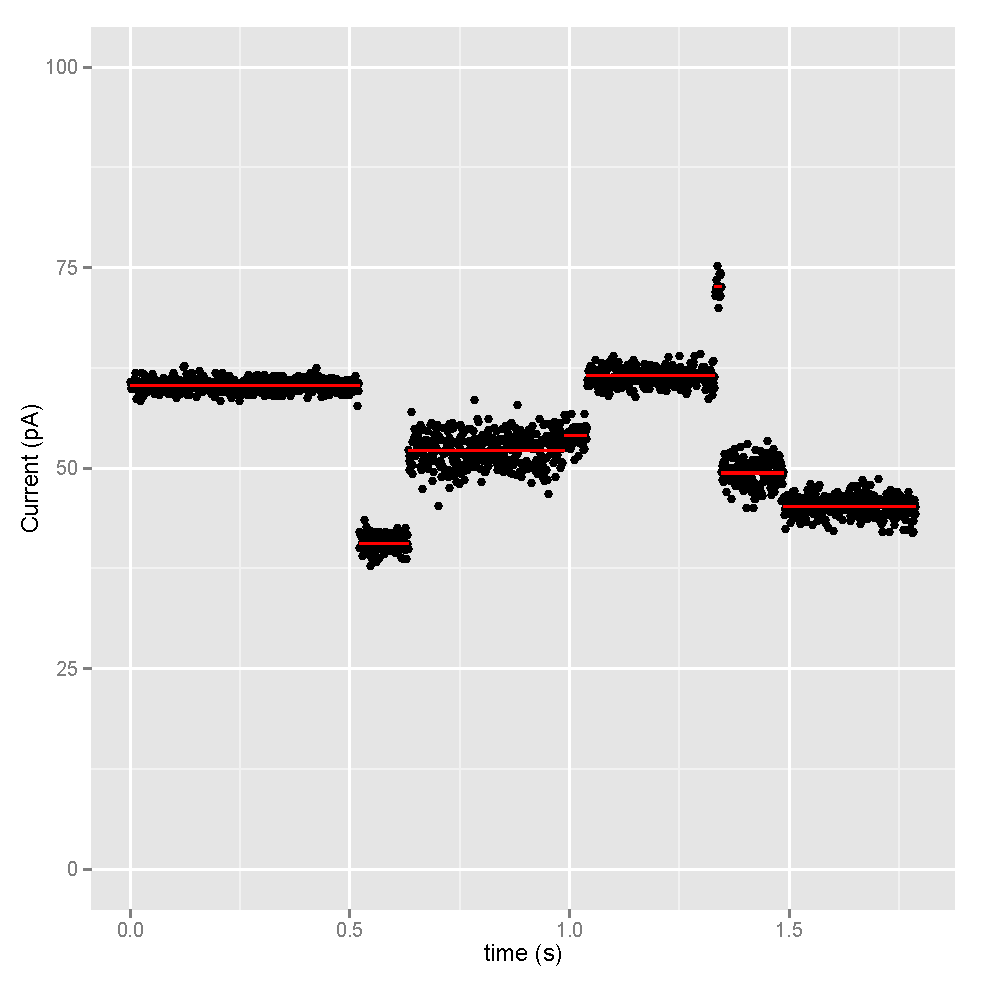
\includegraphics[scale=0.8, clip]{simulation.pdf}}%
	\caption{The black dots show the current samples recorded by the instrument. A single
	red line marks all samples taken from a single $k$-mer (placed at their mean). After each significant jump, it is concluded that a new $k$-mer resides in the pore \citep{simpson}.}
	\label{sampling}
	\end{mdframed}                                                  
\end{figure}  

To help translate events into a DNA sequence, Oxford Nanopore provides a pore model describing the expected current signal for each possible $k$-mer. This comes in the form of $4^k$ normal distributions in a table similar to \ref{poreModel}\footnote{The real table is available at \url{https://github.com/jts/nanopolish/blob/b9dc627e73816a415e4b96b14e8a8bf53622a6c9/etc/r9-models/r9.4_450bps.nucleotide.6mer.template.model}}. The base calling is done by finding the most fitting distribution for each event (based on the distribution calculated from its samples) while taking into account the properties listed earlier.

\begin{table}
	\centering
	\begin{tabular}{l l l l}
		$k$-mer & $\mu$ & $\sigma$  \\	
		\hline{}
		\texttt{AAAAAA} & 66.78 & 3.10  \\
		\texttt{AAAAAC} & 72.67 & 2.19 \\
		\texttt{AAAAAG} & 69.34 & 1.68 \\
		\texttt{AAAAAT} & 70.23 & 0.43 \\
		\texttt{AAAACA} & 67.34 & 1.26 \\
		. . .  & . . . & . . .  \\
		\texttt{TTTTTG} & 87.11 & 2.88 \\
		\texttt{TTTTTT} & 96.89 & 3.60 \\
	\end{tabular}
	\caption{A possible pore model for $6$-mers (as in our case). The table has a total of $4^6 = 4069$ rows, one for every possible $6$-mer. The numbers are made up for illustration purposes. As an example, the samples taken for the $6$-mer \texttt{AAAAAA} is are expected to be drawn from the distribution $\mathcal{N}(66.78, 3.10)$ \citep{simpson}.}.
	\label{poreModel}
\end{table}

\subsection{The Eventalign Algorithm}
As opposed to most approaches which align two DNA sequences to each other, eventalign maps 
the signal data emitted by a nanopore to a reference genome. The algorithm is based on a hidden Markov model which uses the provided reference sequence as its backbone. It depends on an existing base space alignment between the read and the reference. On a high level, it takes the following data:
\begin{enumerate}
	\item A set of raw read signals (HDF5)
	\item The corresponding base called strings for the reads (FASTA or FASTQ)
	\item A reference string
	\item An alignments between the read strings (2) and the reference string (3) (BAM)
\end{enumerate}
It then re-aligns the reads in event space and produces a text representation of the alignments.
\subsection{The Eventalign Output Format}
Eventalign's output comes in a form of a single space delimited text file containing all relevant data. Each row represents one alignment whose data is split into columns. These columns are listed and briefly explained in the table \ref{nanopolishOutput}.

\begin{table}
	\centering
	\begin{tabular}{l|p{10cm}}
		Column name & Explanation\\
		\hline
	\texttt{contig} & The name of the contig the event was aligned to. \\
	\texttt{position} & The position inside the contig. A missing position indicates that the concerned part of the reference wasn't successfully mapped to the signal. \\
	\texttt{reference\_kmer} & The $k$-mer found at this position. \\       
	\texttt{read\_index} & The contig's index. This depends on the nanopolish's internal workings and the number is mostly insignificant. \\
	\texttt{strand}  & The strand indicator. Possibly contains spurious data. A better approach if to compare the \texttt{reference\_kmer} against the \texttt{model\_kmer}. \\
	\texttt{event} &  The event's index in the HDF5 file, indices are assigned sequentially, see \ref{sequencing}\\
	\texttt{event\_level\_mean} & The mean extracted from the event's samples (see \ref{sequencing}). \\
	\texttt{event\_stdv} & The standard deviation extracted from the event's samples (see \ref{sequencing}). \\
	\texttt{event\_length} & The time interval over which all of the event's samples were collected. \\
	\texttt{model\_kmer} & The $k$-mer from the pore model table found to be most fitting to the distribution of the measured samples (see \ref{sequencing} and table \ref{poreModel}). \\
	\texttt{model\_mean} & The samples for the \texttt{model\_kmer} are expected to be drawn from a normal distribution with this mean (table \ref{poreModel}). \\
	\texttt{model\_stdv} & The samples for the \texttt{model\_kmer} are expected to be drawn from a normal distribution with this standard deviation (table \ref{poreModel}) \\
	\texttt{standardized\_level} & dario Računa se po formuli koju je Dario napisao na slack. Ja ne znam ovo objasnit, znas ti? \\
	\texttt{start\_index} & The index of the first sample contained in the event. \\               
	\texttt{end\_index} & The first index after the last sample contained in the event. \\
	\texttt{samples} & All of the event's samples ($\texttt{end\_index} - \texttt{start\_index}$ in total).     
	\end{tabular}
	\caption{The column data eventalign reports for each found alignment. The last three columns are available only if additional sampling data was saved to the HDF5 file. The index in the reference is unambiguously determined by the \texttt{position} and the \texttt{contig}.}
	\label{nanopolishOutput}
\end{table}

\chapter{Protobuf}
\section{General Information}
\textit{Protocol Buffers (Protobuf)}\footnote{\url{https://developers.google.com/protocol-buffers/}} is a method of serializing structured data. It involves an interface description language that describes the structure of some data and a program that generates source code from said description for generating or parsing a stream of bytes that represents the structured data.

Google developed Protocol Buffers for use internally and has provided a code generator for multiple languages under an open source license \citep{protobuf}.
\section{The Specification}
We created a protobuf message specification for easier access to nanopolish 
output data. Protobuf is used to serialize and retrieve structured data.
The protobuf fields correspond with the nanopolish output format. 

\begin{lstlisting}
syntax = "proto3";

package nanopolish;

message EventAlign {
	string contig = 1;
	uint64 position = 2;
	string reference_kmer = 3;
	uint32 read_index = 4;
	// True if strand == 't'
	bool strand = 5;

	string model_kmer = 6;
	double model_mean = 7;
	double model_stdv = 8;

	message Event {
		uint32 index = 1;
		double level_mean = 2;
		double stdv = 3;
		double length = 4;

		double standardized_level = 5;
		uint32 start_idx = 6;
		uint32 end_idx = 7;

		repeated double samples = 8;
	}

	repeated Event events = 10;
}

message NanopolishData {
	repeated EventAlign event_aligns = 1;
}
\end{lstlisting}


\chapter{The Program}
\section{Program specification}
The program 
\footnote{https://github.com/sodic/seminar/tree/master/src}
was designed to enable easier manipulation of nanopolish eventalign 
output data. It can parse the text output from nanopolish, serialize it as protobuf and 
deserialize the protobuf to access the data. It was written in Python 3.6x and
depends on the two non-built-in modules (both can be installed using \texttt{pip}):
\begin{enumerate}
	\item numpy
	\item protobuf
\end{enumerate}
 If you wish to change the protobuf message
specification, you must install the protocol buffer compiler for Python 3
\footnote{https://github.com/protocolbuffers/protobuf}.
Otherwise, you can use the \textit{nanopolish\_pb2.py} file which was generated from
\textit{nanopolish.proto}.

\subsection{Usage}
The program consists of two classes: \textit{NanopolishOutputParser.py} and 
\textit{NanopolishOutputData.py}. The former can parse nanopolish 
eventalign text output and write a protobuf serialization string into a file, while
the latter is an interface for accessing the nanopolish eventalign output data. It requires 
a file path to protobuf serialized data and offers methods for data retrieval. 
A usage example is given below. 


\lstset{frame=tb,
	language=Python,
	aboveskip=3mm,
	belowskip=3mm,
	showstringspaces=false,
	columns=flexible,
	basicstyle={\small\ttfamily},
	numbers=none,
	numberstyle=\tiny\color{gray},
	keywordstyle=\color{blue},
	commentstyle=\color{dkgreen},
	stringstyle=\color{mauve},
	breaklines=true,
	breakatwhitespace=true,
	tabsize=3
}

\begin{lstlisting}


import NanopolishOutputParser as nop
import NanopolishOutputData as nod
import sys

if __name__ == '__main__':
# parse nanopolish txt file and serialize it
parser = nop.NanopolishOutputParser(sys.argv[1])
parser.serialize(sys.argv[2])


# read data from protobuf serialization
data = nod.NanopolishOutputData(sys.argv[2])

# iterate through lines
for ea, event in data:
	if ea.position == 3:
		print(event)

print()
print()
# iterate through event_aligns
# Should give same output as previous for loop.
# Every event_align is unique by (position, read_index)
for ea in data.event_aligns:
	if ea.position == 3:
		for event in ea.events:
			print(event)

# data retrieval


# retrieve specific line
# log time
# Prints pair, first element is event align,
# second is specific event on that line.
print(data.get_line(3))

# retrieve specific event_align
# constant time
print(data.event_aligns[1])


print(data.event_aligns[1].events[0].samples)


try:
	print(data.get_reference_kmer(7, 0))
			kmer, mean, stdv = data.get_model(7, 0)
except KeyError:
	print("There is no event align with read_index = 0 && position = 7")

# print all events on event_align with read_index = 0 && position = 9
# raises KeyError if there is no such
print(data.get_events(9))
\end{lstlisting}
\newpage


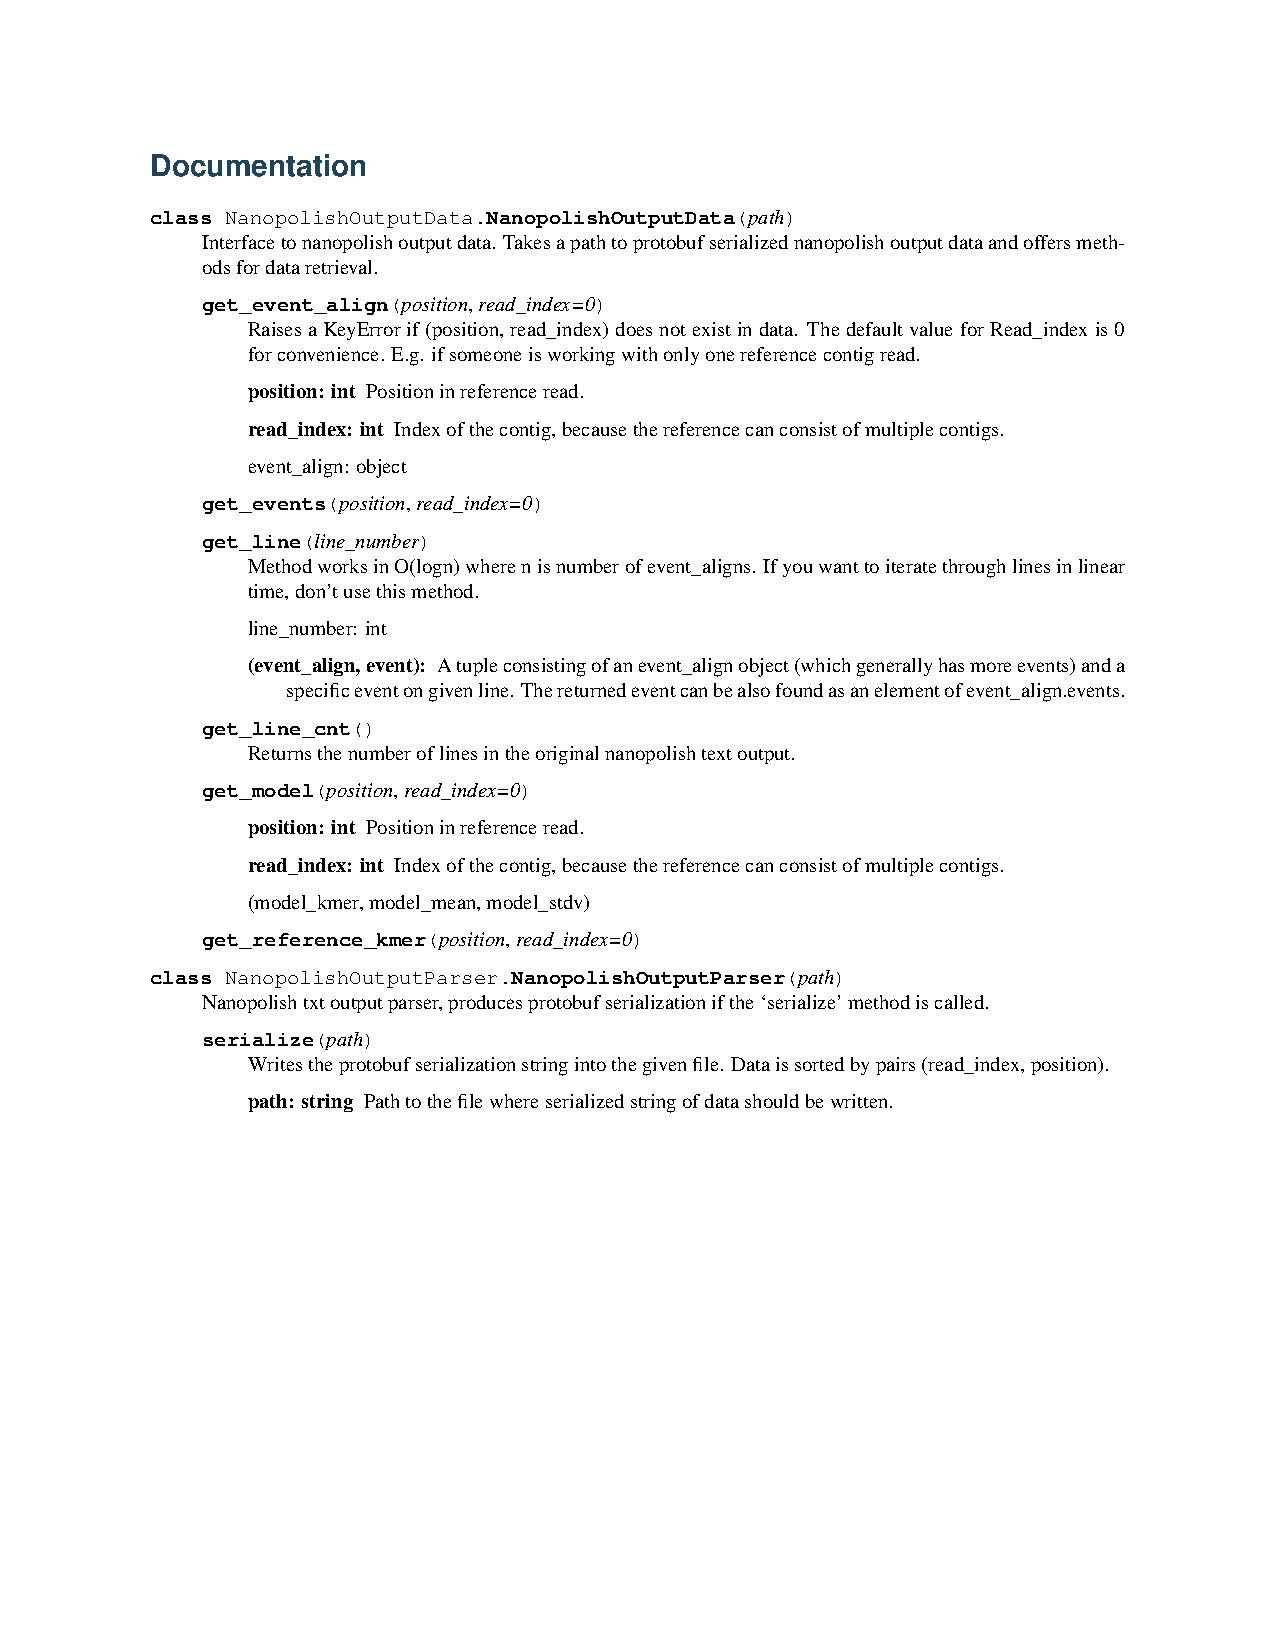
\includepdf[pages=-]{docs.pdf}


\bibliography{literatura}
\bibliographystyle{fer}
\end{document}
